\documentclass{beamer}
\usepackage{pgfpages}
\usepackage[backend=bibtex]{biblatex}
\usepackage{multicol}
\usepackage{multimedia}
\usepackage[absolute,overlay]{textpos}
\usepackage{parskip}
\usepackage{hyperref}
\usepackage{lmodern}
\usepackage{bbding}
\usepackage[absolute,overlay]{textpos}
\usepackage{framed} %Used to shade important equations, color devined with shadecolor
\hypersetup{colorlinks=true, urlcolor=blue}
\setlength{\parskip}{\smallskipamount}
\colorlet{shadecolor}{cyan}
%\usepackage[texcoord,grid,gridunit=mm,gridcolor=red!10,subgridcolor=green!10]{eso-pic} %DELETE when done with grid
\setbeameroption{hide notes} % Only slides
%\setbeameroption{show only notes} % Only notes
%\setbeameroption{show notes on second screen=right} % Both
%\bibliography{../../papers/references.bib}
\setbeamerfont{footnote}{size=\tiny}
%\AtEveryCitekey{\clearfield{title}}

%
% Choose how your presentation looks.
%
% For more themes, color themes and font themes, see:
% http://deic.uab.es/~iblanes/beamer_gallery/index_by_theme.html
%
\mode<presentation>
{
\usetheme{Warsaw}      % or try Darmstadt, Madrid, Warsaw, ...
\usecolortheme{default} % or try albatross, beaver, crane, ...
\usefonttheme{default}  % or try serif, structurebold, ...
\setbeamertemplate{navigation symbols}{}
\setbeamertemplate{caption}[numbered]
} 

\usepackage[english]{babel}
%\usepackage[utf8x]{inputenc} %Doesn't play well with biblatex
\usepackage{amssymb}
\usepackage{bm}
\usepackage{color}
\usepackage{graphicx}
\setbeamercovered{invisible}
\setbeamercovered{%
again covered={\opaqueness<1->{100}}} %This changes the opaqueness of each bullet

\newcommand{\red}[1]{{\color{red}{#1}}}
\newcommand{\checkH}[2]{\begin{textblock*}{1cm}(#1,#2){\Huge \red{\Checkmark}}\end{textblock*}}
\newcommand{\checkh}[2]{\begin{textblock*}{1cm}(#1,#2){\huge \red{\Checkmark}}\end{textblock*}}
\newcommand{\checkL}[2]{\begin{textblock*}{1cm}(#1,#2){\Large \red{\Checkmark}}\end{textblock*}}
\newcommand{\checkl}[2]{\begin{textblock*}{1cm}(#1,#2){\large \red{\Checkmark}}\end{textblock*}}
\renewcommand{\rm}[1]{\mathrm{#1}}

\title[{\color{white}{Chapters 6.1-3}}]{Physics 121: \\ Equilibrium, N2L, Weight}
\author{Cody Petrie}
\institute{Mesa Community College}
\date{}

\begin{document}

%\setbeamertemplate{frametitle}[default][center]
\begin{frame}
\titlepage
\end{frame}

% Uncomment these lines for an automatically generated outline.
%\begin{frame}{Outline}
%  \tableofcontents
%\end{frame}

% Commands to include a figure:
%\begin{figure}
%\includegraphics[width=\textwidth]{your-figure's-file-name}
%\caption{\label{fig:your-figure}Caption goes here.}
%\end{figure}

\begin{frame}{Quiz}
\begin{enumerate}
   \item Which of these is(are) a true statement(s) for mechanical equilibrium? (There may be more than one correct answer)
   \begin{columns}
      \begin{column}{0.5\textwidth}
      \begin{enumerate}
         \item[A.] $\vec{F}_{net} = m\vec{a}$ ($\vec{a} \ne 0$)
         \item[C.] $\vec{F}_{net} = 0$
      \end{enumerate}
      \end{column}
      \begin{column}{0.5\textwidth}
      \begin{enumerate}
         \item[B.] $\vec{a}=0$
         \item[D.] $\vec{v}=0$
      \end{enumerate}
      \end{column}
   \end{columns}
   ~\\~
   \item Consider the situation shown in the figure. What is the acceleration of the box?
   \begin{columns}
   \begin{column}{0.35\textwidth}
   \begin{center}
      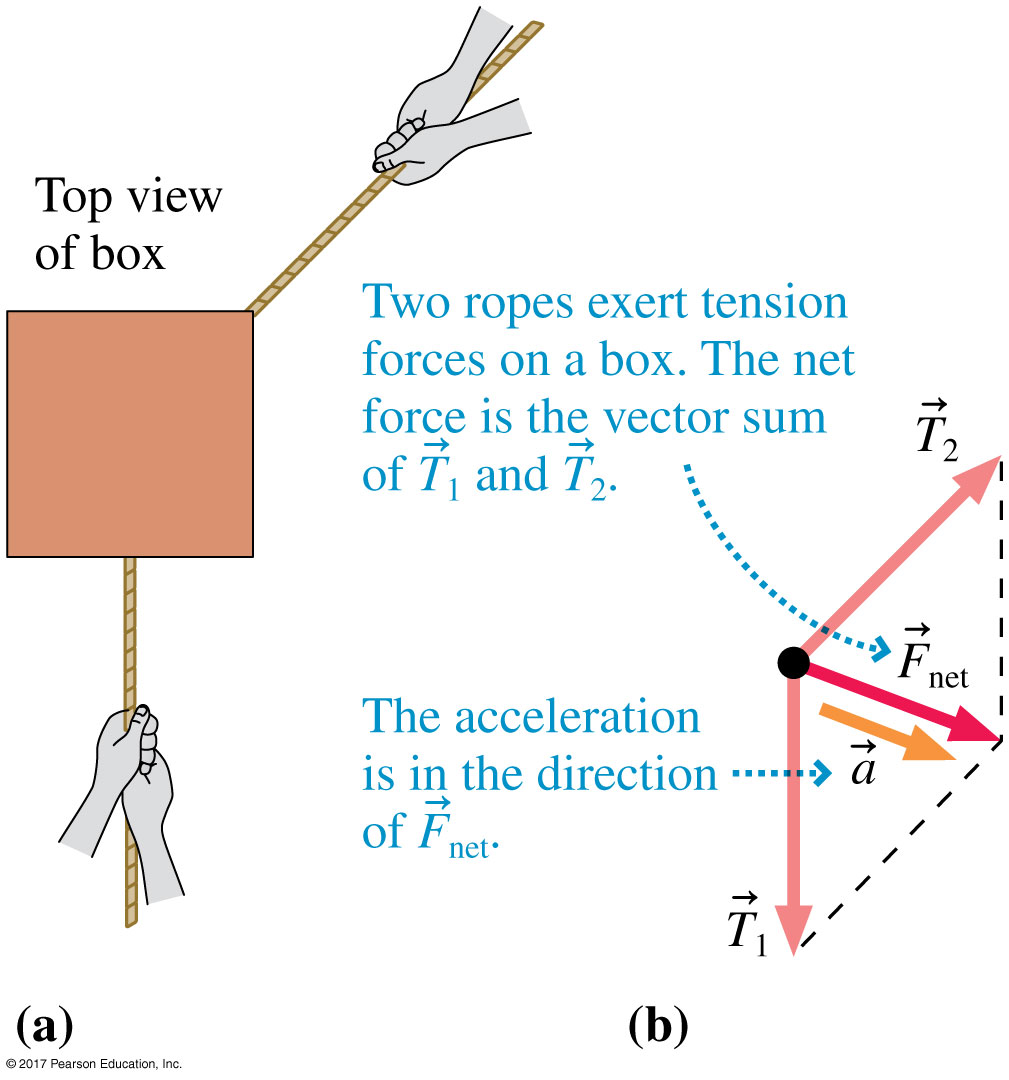
\includegraphics[width=\textwidth]{../figures/05_17_Figure.jpg}
   \end{center}
   \end{column}
   \begin{column}{0.65\textwidth}
   \begin{columns}
   \begin{column}{0.5\textwidth}
   \begin{enumerate}
      \item[A.] $(T_1+T_2)/m$
      \item[C.] 0
   \end{enumerate}
   \end{column}
   \begin{column}{0.55\textwidth}
   \begin{enumerate}
      \item[B.] 9.8 m/s$^2$
      \item[D.] None of the above
   \end{enumerate}
   \end{column}
   \end{columns}
   \end{column}
   \end{columns}
\end{enumerate}
\end{frame}

\begin{frame}{Equilibrium}
\begin{itemize}
   \item When an object is at rest or is moving with constant velocity ($\vec{a}=0$) we say that the object is in mechanical equilibrium.
   \item<2-> That seems like a boring physical system, so why would we want to study it? Can you think of examples of when it might be useful?
   \item<3-> What about engineering stationary objects like bridges?
\end{itemize}
\begin{center}
\uncover<3>{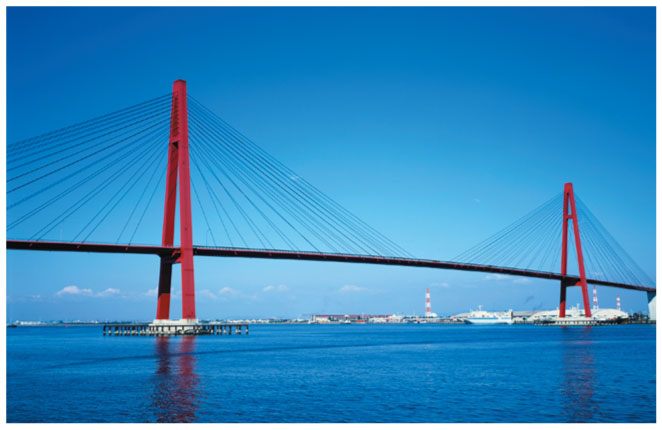
\includegraphics[width=0.7\textwidth]{../figures/06_Pg132_UnFigure.jpg}}
\end{center}
\end{frame}

\begin{frame}{Equilibrium}
\begin{center}
   Write down Newton's second law equation(s) for a 2 dimensional problem in mechanical equilibrium.
\end{center}
\uncover<2>{\begin{align*}
   (F_{net})_x &= \sum\limits_i (F_i)_x = 0 \\
   (F_{net})_y &= \sum\limits_i (F_i)_y = 0
\end{align*}}
\end{frame}

\begin{frame}{Quick Check}
\begin{center}
   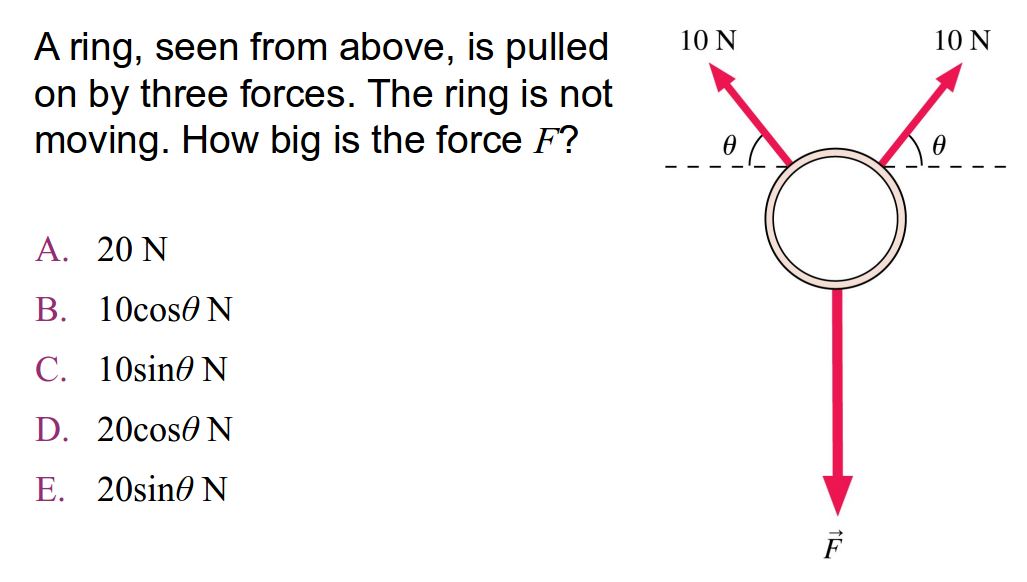
\includegraphics[width=\textwidth]{../figures/QC6_2.png}
\end{center}
\only<2>{\checkL{1.0cm}{6.5cm}}
\end{frame}

\begin{frame}{Example}
   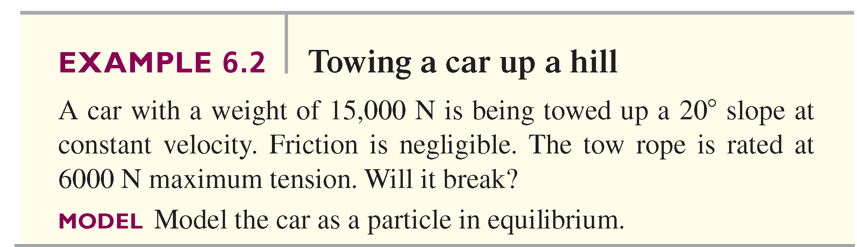
\includegraphics[width=\textwidth]{../figures/example6_2.png} \\~\\
   \begin{center} Draw a picture, build a free body diagram and write down unknowns and things you need to find. \end{center} ~\\
   \uncover<2>{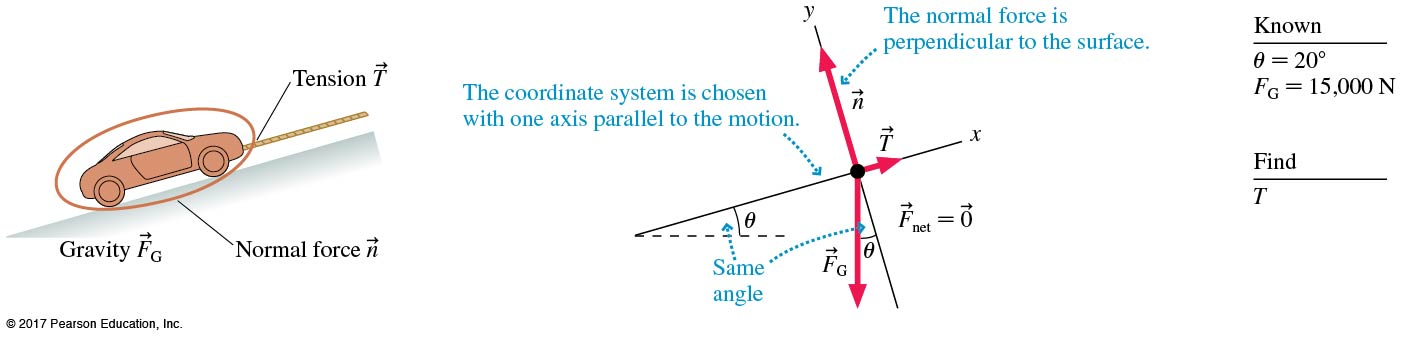
\includegraphics[width=\textwidth]{../figures/06_02_Figure.jpg}}
\end{frame}

\begin{frame}{Example}
\begin{center}
   Now write down the Newton's second law equations
   \uncover<2>{\begin{align*}
      (F_{net})_x &= \sum F_x = T_x + n_x + (F_G)_x = 0 \\
      (F_{net})_y &= \sum F_y = T_x + n_y + (F_G)_y = 0 \\
   \end{align*}}
   \uncover<3>{Now write down what each of these force components are and plug them into Newton's second law equations}
   \uncover<4>{\begin{align*}
      T_x=T, T_y=0, n_x=0, n_y&=n, (F_G)_x = -F_G\sin\theta, (F_G)_y = -F_G\cos\theta \\
      &T-F_G\sin\theta = 0 \\
      &n-F_G\cos\theta = 0
   \end{align*}}
   \uncover<5>{The first equation can be used to solve for the tension
   \begin{equation*}
      T=F_G\sin\theta = (15,000\text{ N})\sin 20^\circ = 5100\text{ N}
   \end{equation*}
   5100 N $<$ 6000 N so {\bf the tow rope holds}!}
\end{center}
\end{frame}

\begin{frame}{Quick Check}
\begin{center}
   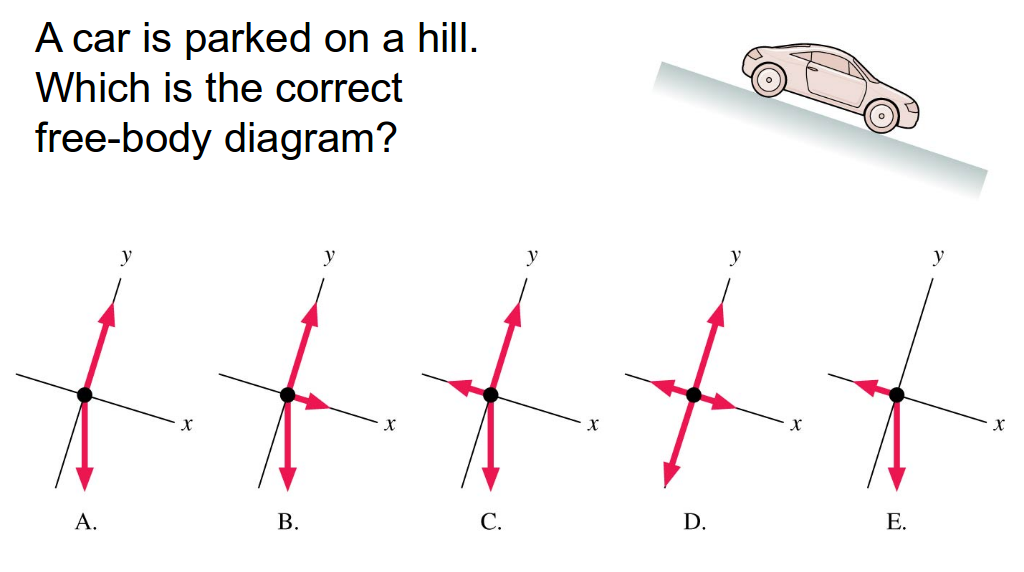
\includegraphics[width=\textwidth]{../figures/QC6_3.png}
\end{center}
\only<2>{\checkL{6.0cm}{7.2cm}}
\end{frame}

\begin{frame}{Quick Check}
\begin{center}
   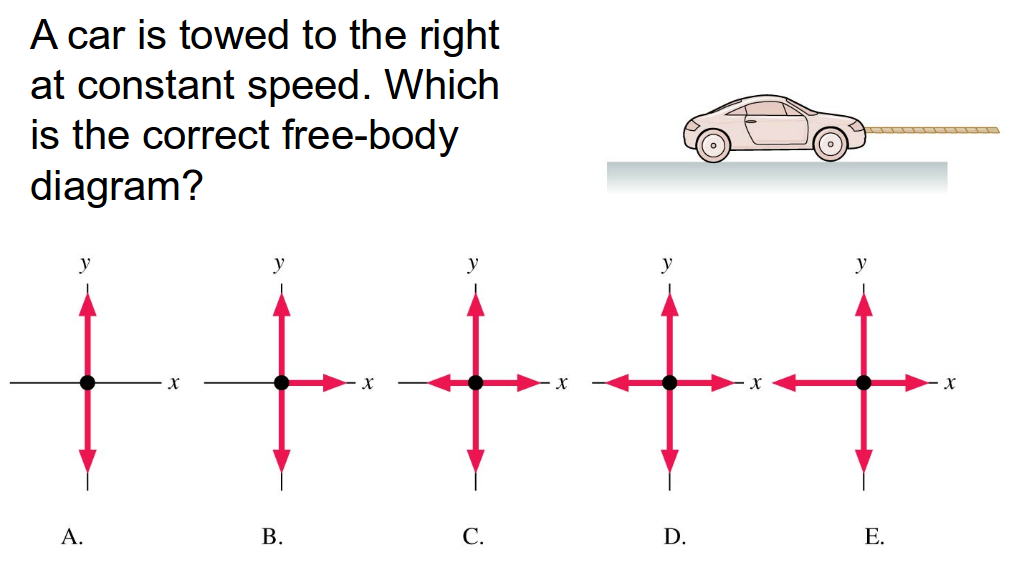
\includegraphics[width=\textwidth]{../figures/QC6_4.png}
\end{center}
\only<2>{\checkL{8.0cm}{7.2cm}}
\end{frame}

\begin{frame}{Using Newton's Second Law}
\begin{itemize}
   \item Alright, now we've been doing a lot stuff that hasn't been connected yet. So how do you use Newton's second law to solve physics problems?
   \item There is a long version is the book that I'll show here and then I'll break it down to the most important parts.
\end{itemize}
\end{frame}

\begin{frame}{Using Newton's Second Law}
\begin{center}
   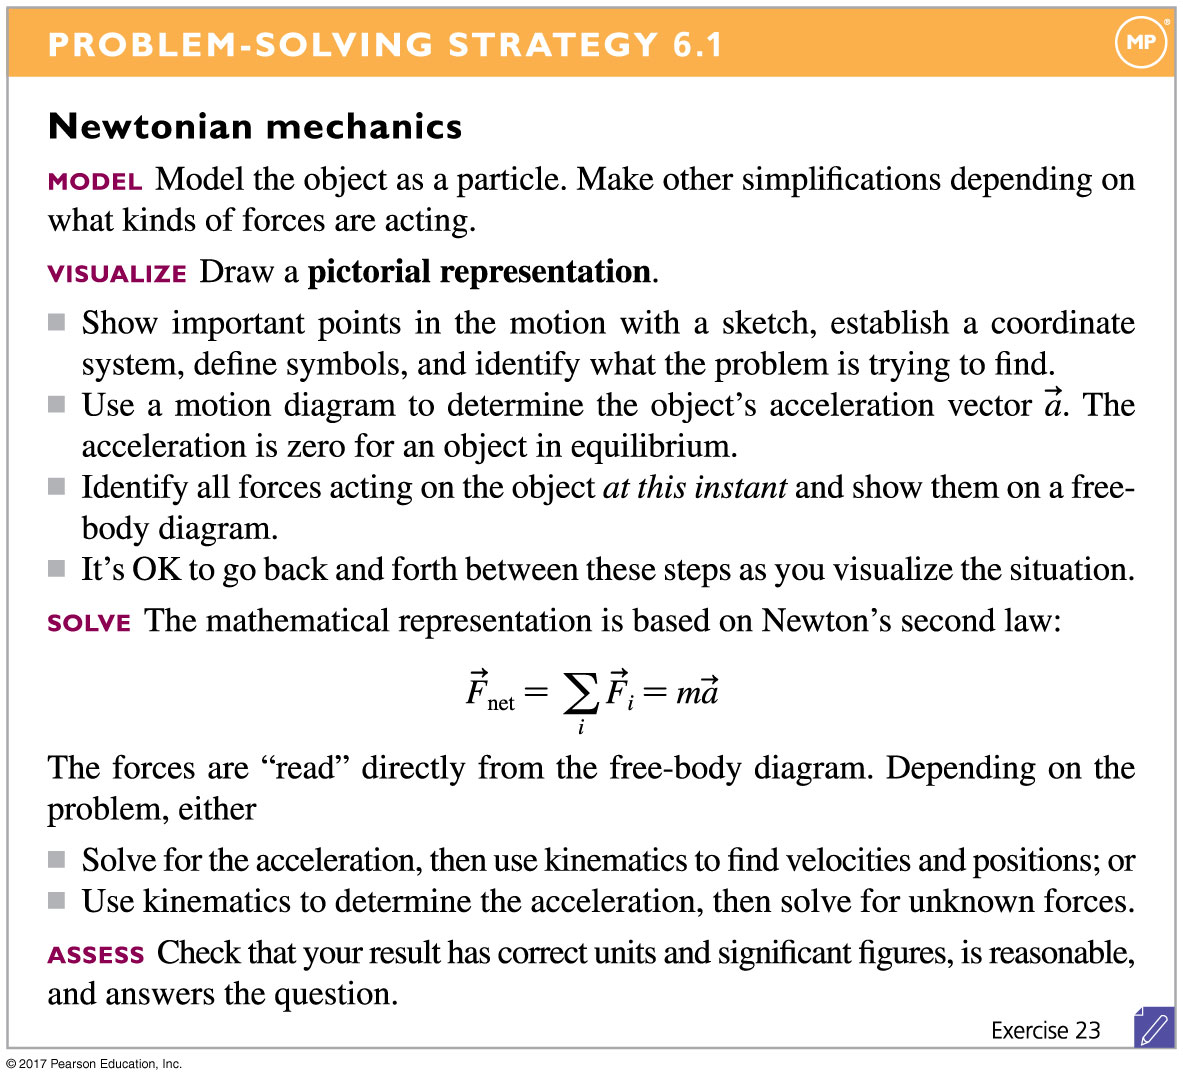
\includegraphics[height=0.93\textheight]{../figures/06_ProblemSolvingStrat_01.jpg}
\end{center}
\end{frame}

\begin{frame}{Using Newton's Second Law}
\begin{enumerate}
   \item Draw a picture.
   \begin{enumerate}
      \item Choose a coordinate system and simplify the model as much as possible (but not more) (particle model)
      \item Make the drawing a free-body diagram including ALL forces acting on the object.
   \end{enumerate}
   \item Write down Newton's second law equation(s)
   \begin{equation*}
      \vec{F}_{net} = \sum\limits_i \vec{F}_i = m\vec{a}
   \end{equation*}
   \item Do one of the following
   \begin{enumerate}
      \item Solve for the acceleration, then use kinematics to find velocities and positions OR
      \item Use kinematics to determine the acceleration, then solve for unknown forces.
   \end{enumerate}
\end{enumerate}
\end{frame}

\begin{frame}{Example}
   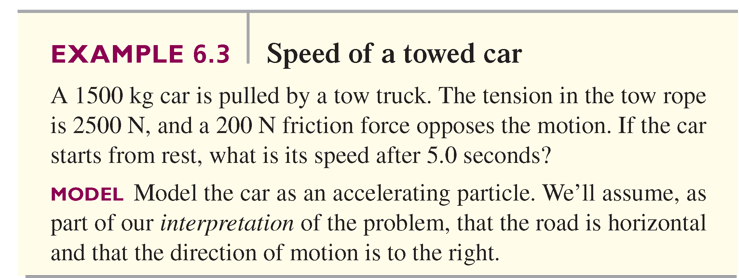
\includegraphics[width=\textwidth]{../figures/example6_3.png} \\~\\
   \only<1>{\begin{center} Draw a picture, build a free body diagram and write down unknowns and things you need to find. \end{center}}
   \uncover<2>{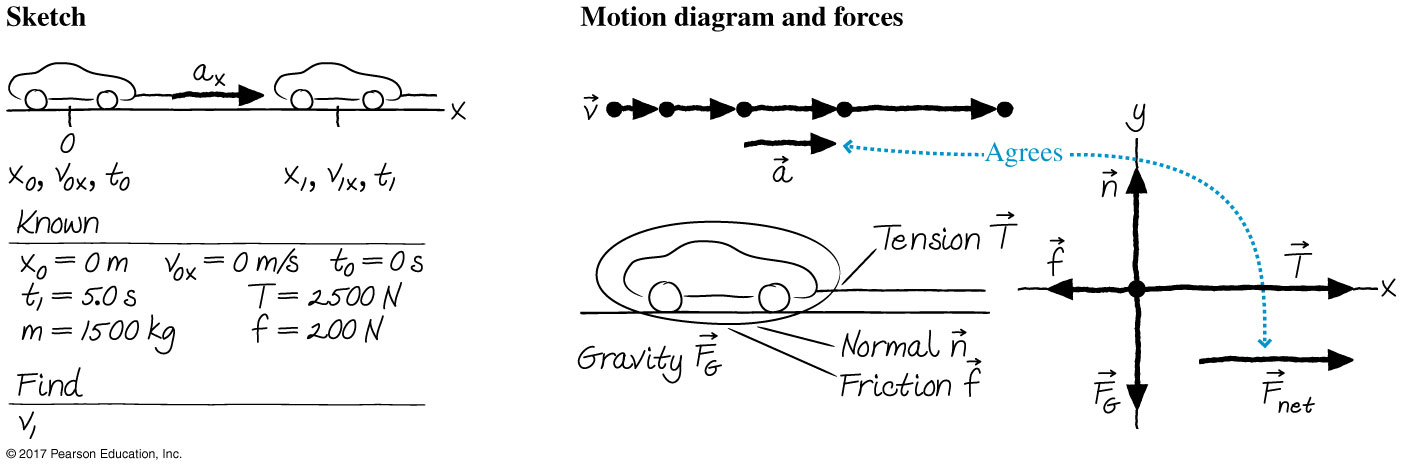
\includegraphics[width=\textwidth]{../figures/06_03_Figure.jpg}}
\end{frame}

\begin{frame}{Example}
\begin{center}
   Now write down the Newton's second law equations
   \uncover<2>{\begin{align*}
      (F_{net})_x &= \sum F_x = T_x + f_x + n_x + (F_G)_x = ma_x \\
      (F_{net})_y &= \sum F_y = T_y + f_y + n_y + (F_G)_y = ma_y \\
   \end{align*}}
   \uncover<3>{Now write down what each of these force components are and plug them into Newton's second law equations}
   \uncover<4>{
   \begin{equation*}
      T_x=+T, T_y=0, n_x=0, n_y=+n
   \end{equation*}
   \begin{equation*}
      f_x=-f, f_y=0, (F_G)_x = 0, (F_G)_y = -F_G
   \end{equation*}
   \begin{align*}
      a_x &= \frac{1}{m}(T-f) \\
         &= \frac{1}{1500\text{ kg}}(2500\text{ N}-200\text{ N}) = 1.53\text{ m/s}^2 \\
      a_y &= \frac{1}{m}(n-F_G)
   \end{align*}}
\end{center}
\end{frame}

\begin{frame}{Example}
\begin{center}
   Now we have the (constant) acceleration and so use kinematics to solve for $v_{1x}$
   \uncover<2>{\begin{align*}
      v_{1x} &= v_{0x}+a_x\Delta t \\
      &= 0+(1.53\text{ m/s}^2)(5.0\text{ s}) = 7.7\text{ m/s}^2 \approx 15\text{ mph}
   \end{align*}
   Is that a reasonable speed to be at after accelerating for 5 s?}
\end{center}
\end{frame}

\begin{frame}{Constant Force}
\begin{center}
   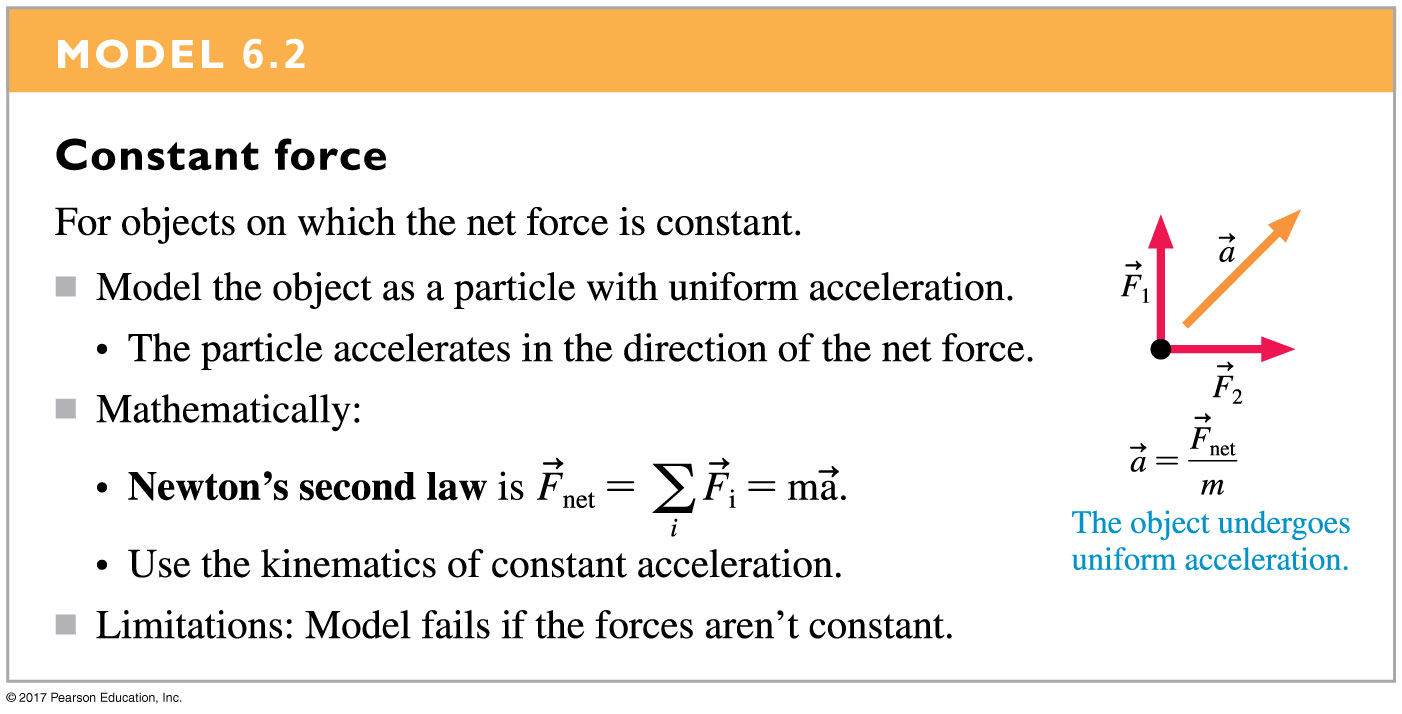
\includegraphics[width=\textwidth]{../figures/06_ModelBox_02.jpg}
\end{center}
\end{frame}

\begin{frame}{Quick Check}
\begin{center}
   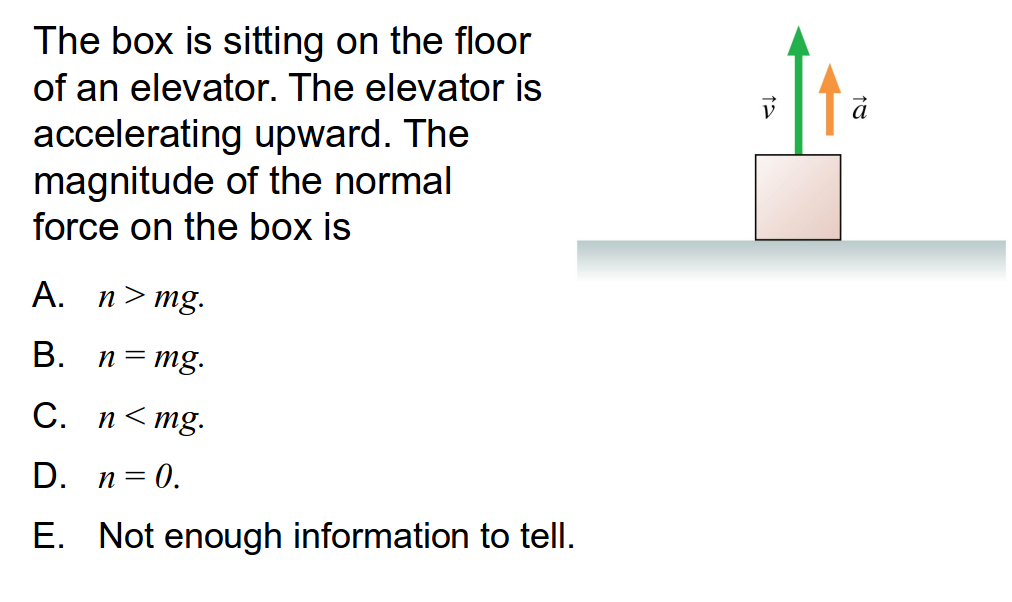
\includegraphics[width=\textwidth]{../figures/QC6_6.png}
\end{center}
\only<2>{\checkL{1.0cm}{4.4cm}}
\end{frame}

\begin{frame}{Mass, Gravity and Weight}
\begin{center}
   \color{blue}{\Huge Mass, Gravity and Weight}
\end{center}
\end{frame}

\begin{frame}{Mass - An Intrinsic Property}
\begin{columns}
\begin{column}{0.5\textwidth}
\begin{itemize}
   \item A pan balance, shown in the figure, is a device for measuring mass.
   \item The measurement does not depend on the strength of gravity.
   \item Mass is a scalar quantity that describes an object's inertia.
   \item Mass describes the amount of matter in an object.
   \item Mass is an intrinsic property of an object.
\end{itemize}
\end{column}
\begin{column}{0.5\textwidth}
   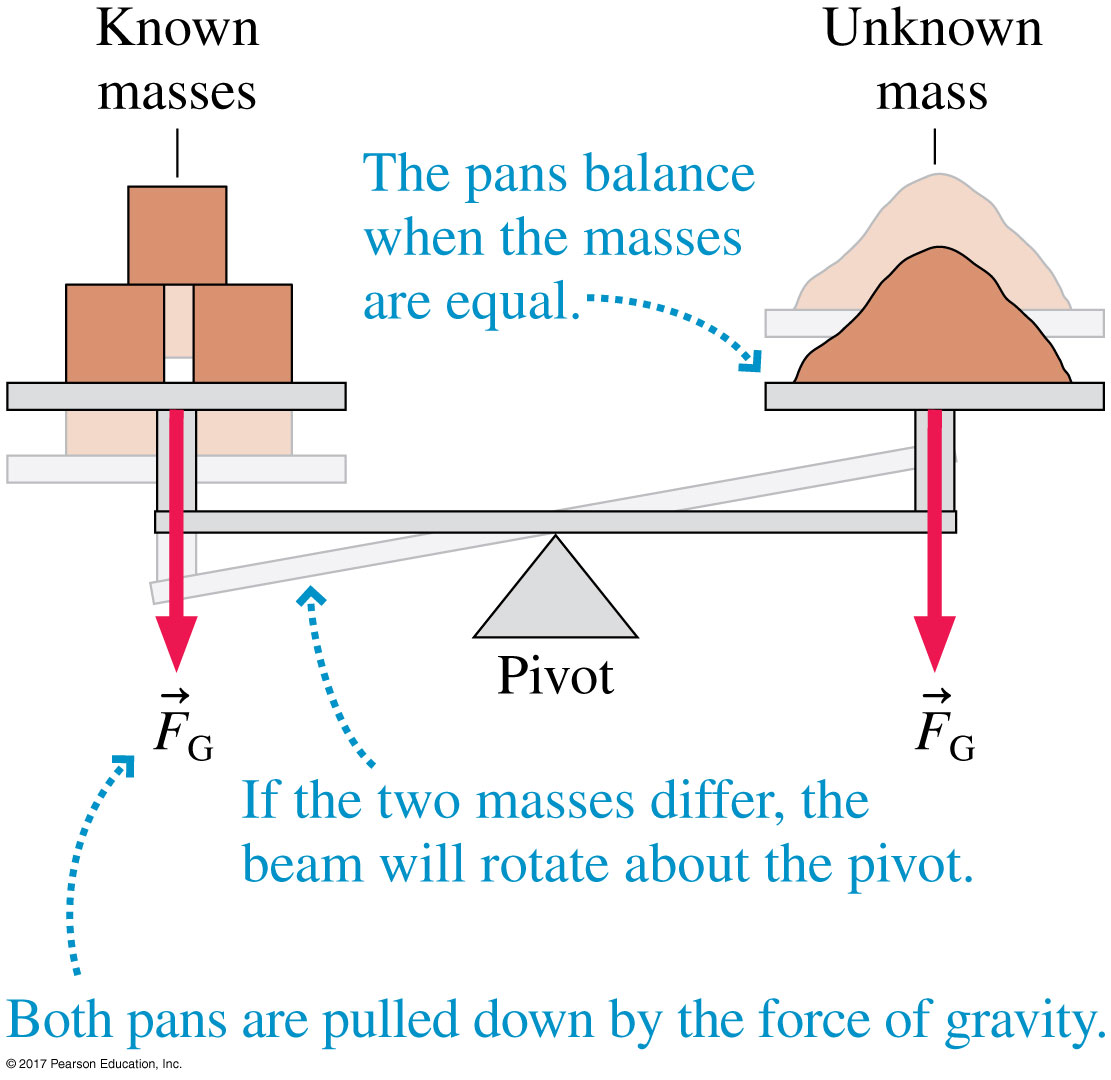
\includegraphics[width=\textwidth]{../figures/06_05_Figure.jpg}
\end{column}
\end{columns}
\end{frame}

\begin{frame}{Gravity - A Force}
\begin{center}
   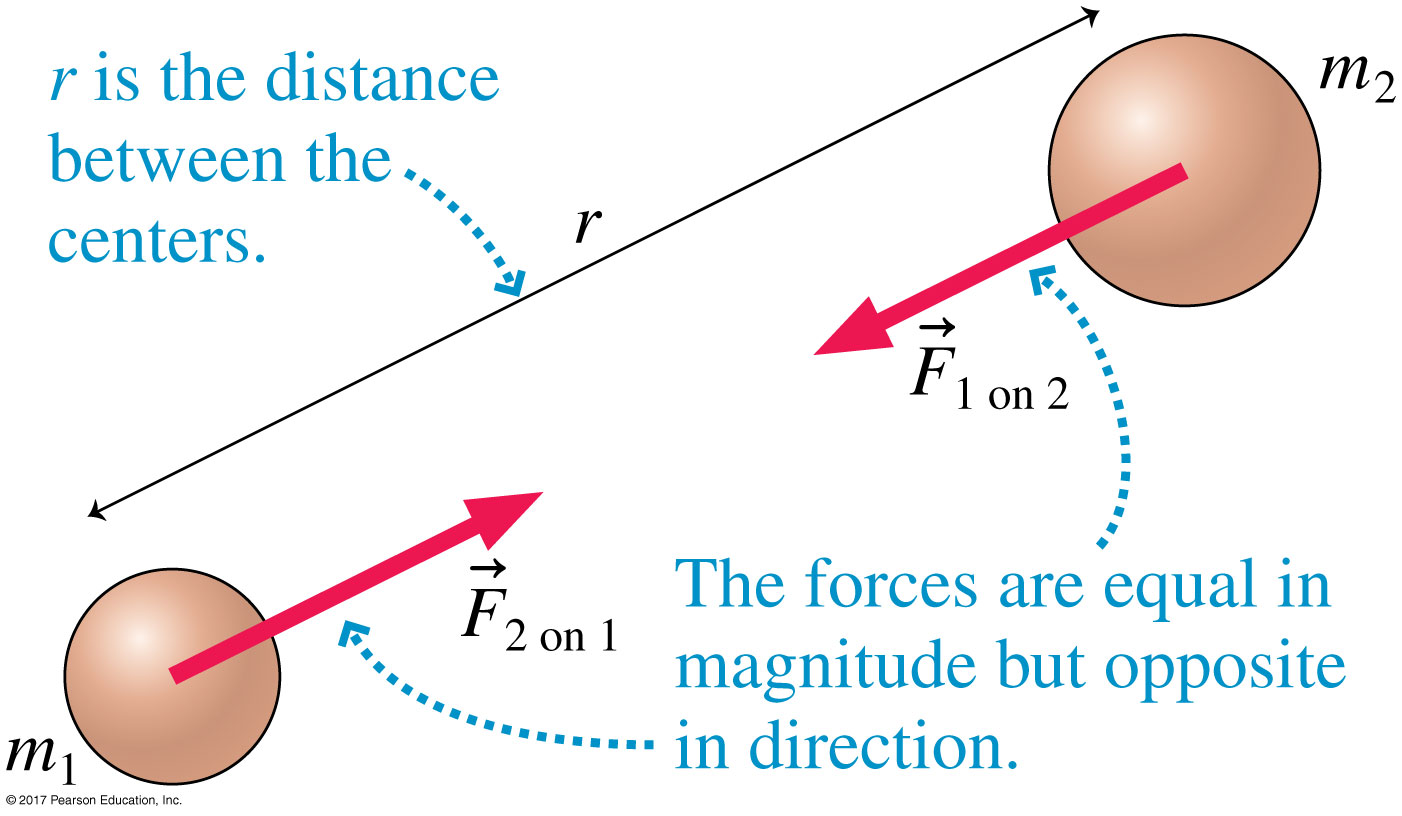
\includegraphics[width=0.5\textwidth]{../figures/06_06_Figure.jpg}
\end{center}
\begin{itemize}
   \item Gravity is an attractive, long-range force between any two objects.
   \item The figure shows two objects with masses $m_1$ and $m_2$ whose centers are separated by distance $r$.
   \item Each object pulls on the other with a force:
   \begin{equation*}
      F_{12} = F_{21} = \frac{Gm_1m_2}{r^2} ~(\text{\bf Newton's Law of Gravity})
   \end{equation*}
   where $G = 6.67\times10^{-11}$ Nm$^2$/kg$^2$ is the gravitational constant.
\end{itemize}
\end{frame}

\begin{frame}{Gravity - A Force}
\begin{itemize}
   \item Why does it seem that there is no gravitational force between any two of us?
   \item<2-> There is, it's just very small compared to other factors.
   \item<3-> For an object of mass $m$ near the surface of the earth the gravitational force from a planet with mass $M$ and radius $R$ is
   \begin{equation*}
      \vec{F}_G = \vec{F}_{\text{planet on }m} = \left(\frac{GMm}{R^2},\text{ down}\right) = (mg,\text{ down})
   \end{equation*}
   \item<4-> Notice that the acceleration due to gravity $g$ doesn't depend on the mass of the object $m$, so it's always constant assuming the mass and radius of the planet don't change \ldots EVERYTHING FALLS AT THE SAME RATE, and now you know why $:)$
   \item<5-> Show this\ldots \uncover<6>{For earth $g=\frac{GM}{R^2} = 9.8$m/s$^2$.}
\end{itemize}
\end{frame}

\begin{frame}{Weight - A Measurement}
\begin{itemize}
   \item Weight is a measurement of gravitational force.
   \item It is usually measured by measuring another force that is equal to the gravitational force with $\vec{a}=\vec{F}_{net} = \vec{0}$ (think Newton's 2st law and equilibrium $:)$)
\end{itemize}
\begin{center}
   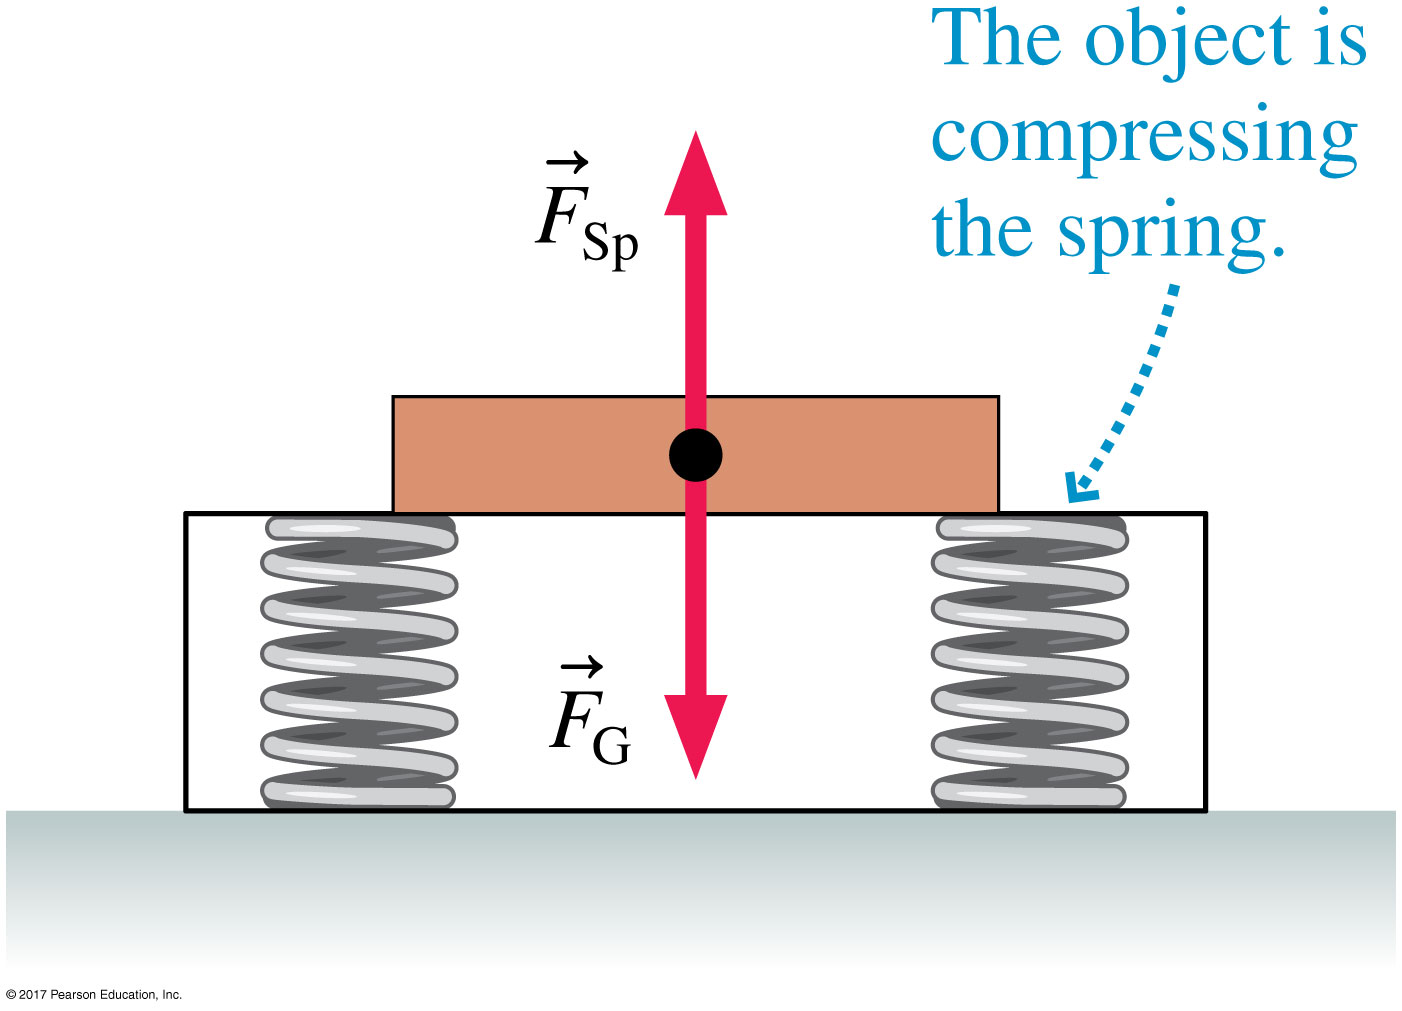
\includegraphics[width=0.5\textwidth]{../figures/06_09_Figure.jpg}
\end{center}
\end{frame}

\begin{frame}{Quick Check}
\begin{center}
   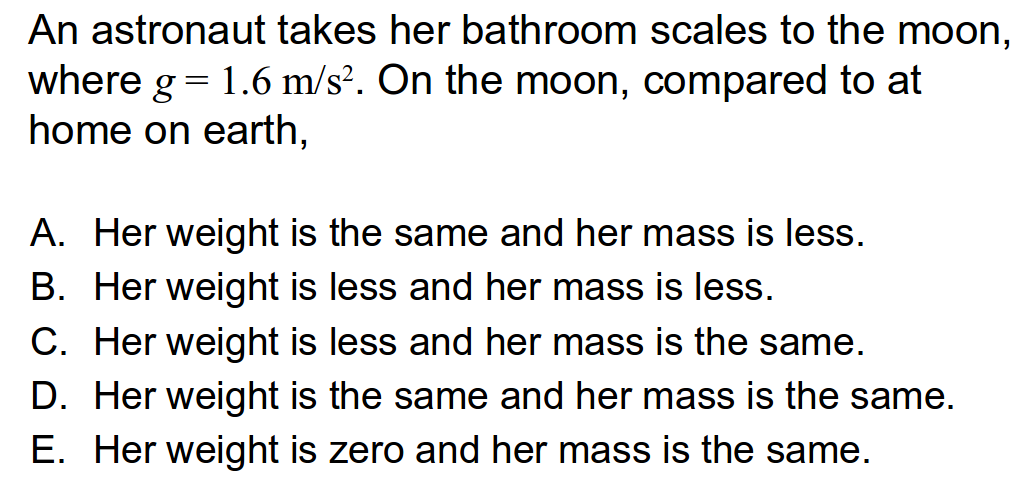
\includegraphics[width=\textwidth]{../figures/QC6_7.png}
\end{center}
\only<2>{\checkL{1.0cm}{5.3cm}}
\end{frame}

\begin{frame}{Quick Check}
\begin{center}
   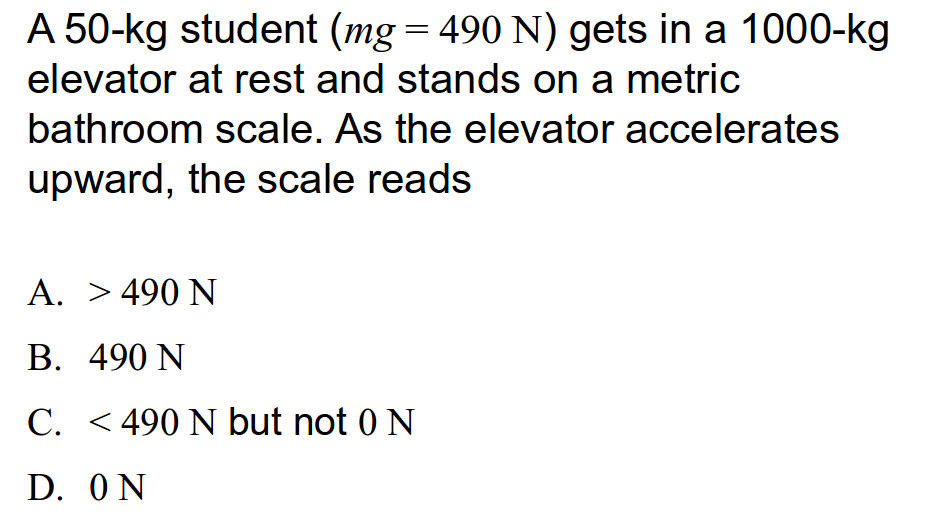
\includegraphics[width=\textwidth]{../figures/QC6_8.png}
\end{center}
\only<2>{\checkL{1.0cm}{4.8cm}}
\end{frame}

\begin{frame}{Quick Check}
\begin{center}
   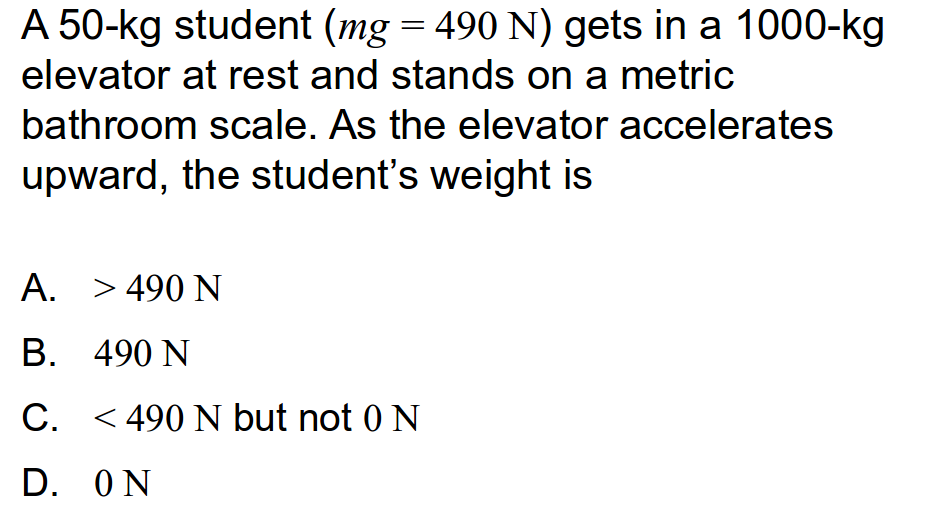
\includegraphics[width=\textwidth]{../figures/QC6_9.png}
\end{center}
\only<2>{\checkL{0.9cm}{4.7cm}}
\end{frame}

\begin{frame}{Weightlessness}
\begin{itemize}
   \item What if the cable breaks and the student falls with acceleration $a_y=-g$. What would be the student weight?
   \item<2-> $w=0$ N??? They are weightless, but they are still on earth? They still weight SOMETHING right? Is that right or is something wrong?
\end{itemize}
\end{frame}

\begin{frame}{Weightlessness}
\begin{itemize}
   \item That is in fact true, an object in free fall has no weight. This is the case for astronauts as well.
\end{itemize}
\begin{center}
   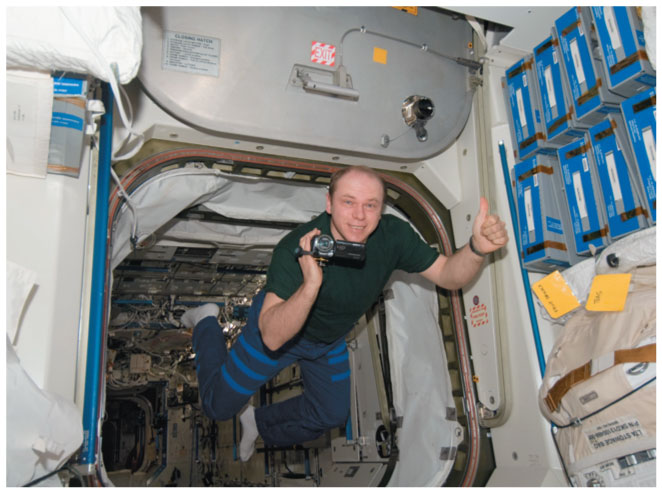
\includegraphics[width=0.5\textwidth]{../figures/06_Pg140_UnFigure.jpg}
\end{center}
\begin{itemize}
   \item In fact $g_{iss} \approx 8.7$m/s$^2$ and $g_{moon} \approx 1.6$m/s$^2$ so they should fall right? They do fall, orbiting objects are in ``free fall" and are thus weightless.
\end{itemize}
\end{frame}

\begin{frame}{Quick Check}
\begin{center}
   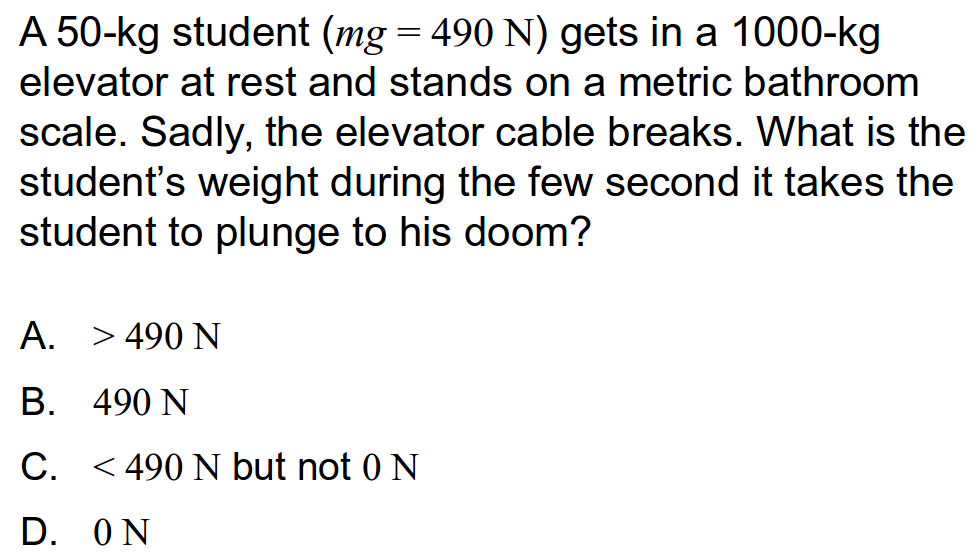
\includegraphics[width=\textwidth]{../figures/QC6_10.png}
\end{center}
\only<2>{\checkL{0.9cm}{7.2cm}}
\end{frame}

\begin{frame}{Quick Check}
\begin{center}
   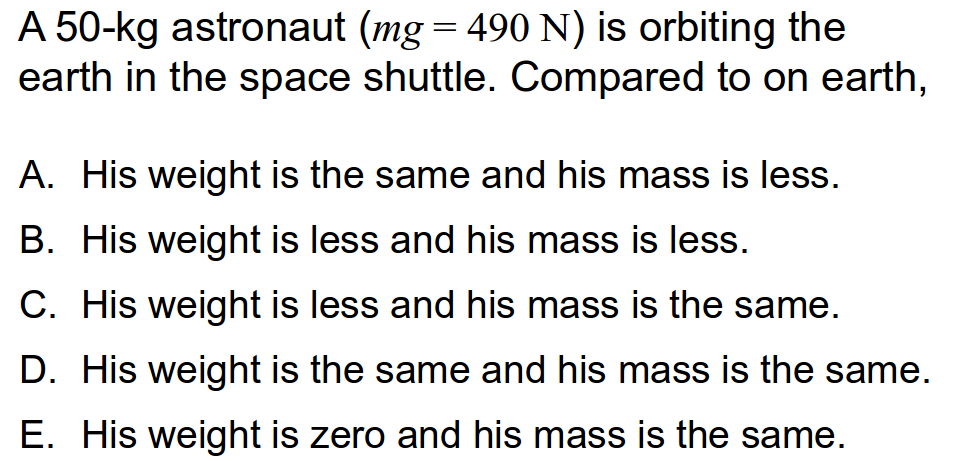
\includegraphics[width=\textwidth]{../figures/QC6_11.png}
\end{center}
\only<2>{\checkL{0.9cm}{6.6cm}}
\end{frame}

\begin{frame}{Picture References}
\tiny
Nothing this time
\end{frame}

\end{document}
